
\chapter{太陽光発電データの時刻補正手法}
\label{chap:second}

\section{緒言}
本章では, 太陽光発電データの計測時刻の補正手法を提案する.

% 20220523

\section{太陽光発電の計測データの問題点について}
本研究で管理している太陽光発電データは, データを計測しているPCの内部時計が標準時刻とずれているため, 他地点で計測しているデータと時刻同期ができない問題があった. 

そこで, 時刻がずれていない実測値と, 計算式により求まる大気外日射量との間の時間的遅延の秒数を相互相関を用いて求めることで, 実測値を標準時に補正する.

\section{大気外日射量の計算式}
任意の緯度経度, 時刻における大気外日射量$Q$は, 任意の緯度$\phi$, 経度$\lambda$の地点における任意の時刻, 太陽高度$\alpha$から求めることができる.

まず, 次式より元旦からの通し日数$dn$に基いて定めた$\theta$を用いて, 当該日の太陽赤緯$\delta$, 地心太陽距離$\frac{r}{r^{*}}$, 均時差$E_q$をそれぞれ以下の式により求める.
\begin{eqnarray}
  \theta =  \frac{2\pi (dn-1)}{365}
\end{eqnarray}

\begin{eqnarray}
  \begin{split}
    \delta =  0.006918-0.399912\cos \theta+0.070257\sin \theta-0.006758\cos 2\theta\\
    +0.000907\sin 2\theta-0.002697\cos 3\theta+0.001480\sin 3\theta
  \end{split}
\end{eqnarray}

\begin{dmath}
  \frac{r}{r^{*}} =  \frac{1}{\sqrt{1.000110+0.034221\cos \theta+0.001280\sin \theta+0.000719\cos 2\theta+0.000077\sin 2\theta}}
\end{dmath}

\begin{eqnarray}
  \begin{split}
    E_q =  0.000075+0.001868\cos \theta-0.032077\sin \theta\\
    -0.014615\cos 2\theta-0.040849\sin 2\theta
  \end{split}
\end{eqnarray}

日本標準時間から, 太陽の時角$h$を求める.

\begin{eqnarray}
  h = \frac{(日本標準時間-12)\pi}{12}+標準子午線からの経度差+E_q
\end{eqnarray}

$\delta$, $\phi$, $h$の値が既知となったので$\alpha$は

\begin{eqnarray}
  \alpha = \arcsin (\sin \phi\sin \delta+\cos \phi\cos \delta\cos h)
\end{eqnarray}

により求まる.

最後に, $Q$が

\begin{eqnarray}
  Q = 1367(\frac{r^{*}}{r})^{2}\sin \alpha
\end{eqnarray}

により求まる. 1367\si{\watt}/\si{\metre\squared}は太陽定数である.

式(2.1)~式(2.7)を用いることで, 任意の緯度経度, 時刻における大気外日射量が求まる.

% 20220529

\subsection{実測値と大気外日射量との比較}
Elasticsearchサーバーから取得した2022年6月2日のリサイクル館の実測値と, 計算式から求めた大気外日射量を図\ref{20220529-p1}に示す. 実測値は地表に設置された太陽光パネルが計測したものであるのに対して, 大気外日射量は地球大気の上端(約8km上空)で受け取る日射量を計算したものであるため, 一日を通して最大となる日射量の大きさに差がある.

なお, 図\ref{20220529-p1}は\texttt{python3 calc_corr.py -dt 2022/06/02 -surface_tilt 22 -surface_azimuth 179 -show_graph}コマンドを実行してプロットしている.

\begin{figure}[H]
  \hspace*{-1cm}
  \centering
  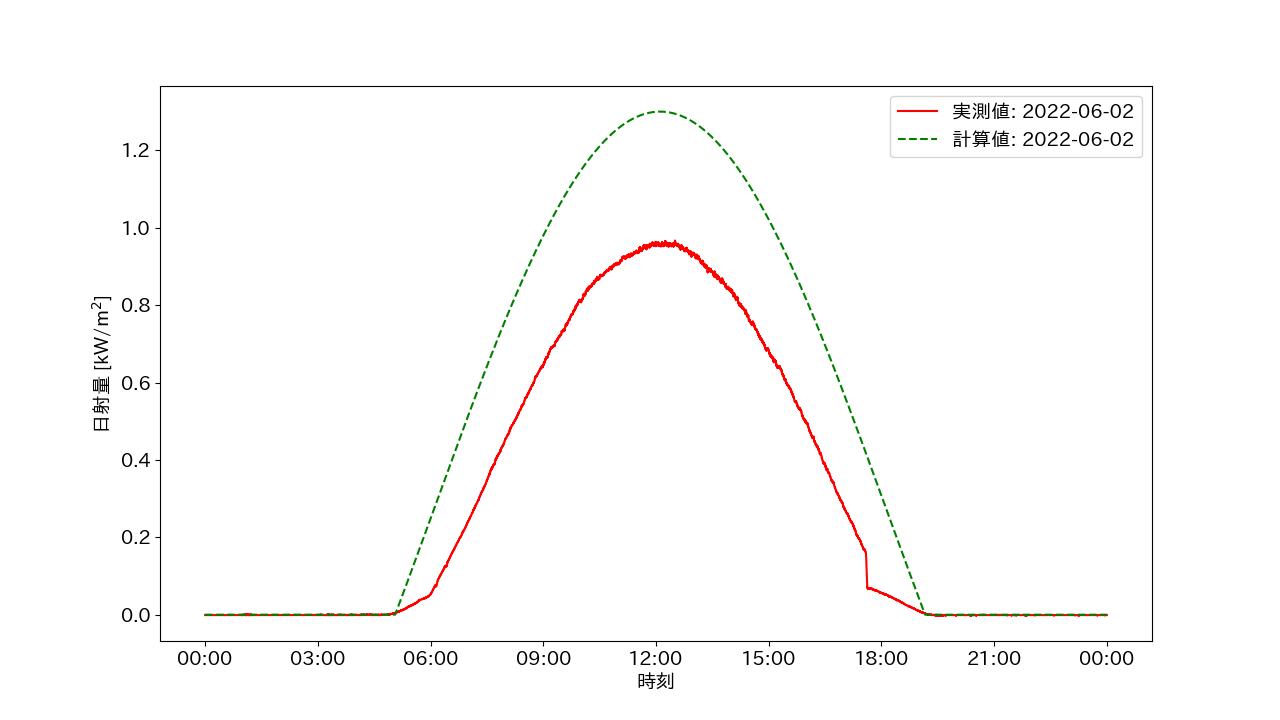
\includegraphics[width=160mm]{sotu/figure/2/original-20220602-corr.png}
  \caption{2022年6月2日の実測値と大気外日射量(式(2.7))}
  \label{20220529-p1}
\end{figure}

% 20220620

\subsection{相互相関による時刻補正法}
相互相関の計算に使用するデータの計測期間を, 快晴だった2022年6月2日0時0分から2022年6月2日23時59分までとした. なお, 使用したデータはリサイクル館で計測し, インターネット時刻に同期したタイムスタンプを計測時刻としている.

同じ期間の大気外日射量を式(2.7)で求め, 実測値との相互相関を計算した結果, 実測値を124秒遅らせると, 相関が最大となった. また, 同様に快晴であった2022年5月3日と2022年5月18日ではそれぞれ39秒, 71秒遅らせた際に相関が最大となり, 3日間の平均値は78秒であった.

使用した実測値はインターネット時刻に同期しているので, 遅れ時間は0秒となるのが正しいにも関わらず平均78秒となったのは, 地表日射量ではなく大気外日射量を使用したためと考えられる.

\section{地表日射量の予測}

地表日射量の予測を行うため, 式(2.1)~式(2.7)を使った方法ではなく, pvlibライブラリ\cite {2}を使用して地表日射量を求め, 相互相関を計算した.

\subsection{pvlibの概要}
pvlibは, 太陽光発電システムの性能シミュレーションや関連するタスクを実行するための関数とクラスのセットを提供するライブラリである. 

以下は, pvlibの主な特徴である.

\begin{itemize}
  \item 太陽位置計算: pvlibは, 地球上の任意の場所における太陽の位置を計算する機能を提供する. これは, 太陽の方位角や高度角を求めるのに使用される.
  \item 大気透過モデル: 大気を通過する太陽放射の量や質を推定するモデルが含まれている.
  \item 太陽光発電システムの性能モデリング: 太陽光発電モジュールやインバーターの性能モデルが含まれており, これらの条件下での太陽光発電システムの出力をシミュレートできる.
\end{itemize}

\subsection{実測値とpvlibにより求まる地表日射量の比較}
Elasticsearchサーバーから取得したリサイクル館の実測値と, pvlibを用いて求めた地表日射量との比較を図\ref{2-p1}に示す.

なお, 図\ref{2-p1}は\texttt{python3 calc_corr.py -dt 2022/06/02 -surface_tilt 22 -surface_azimuth 179 -show_graph}コマンドを実行してプロットしている.

図\ref{2-p1}と図\ref{20220529-p1}と比較すると, 大気外日射量より地表日射量の方が実測値により近い概形となっていることが分かる.

\begin{figure}[H]
  \hspace*{-1cm}
  \centering
  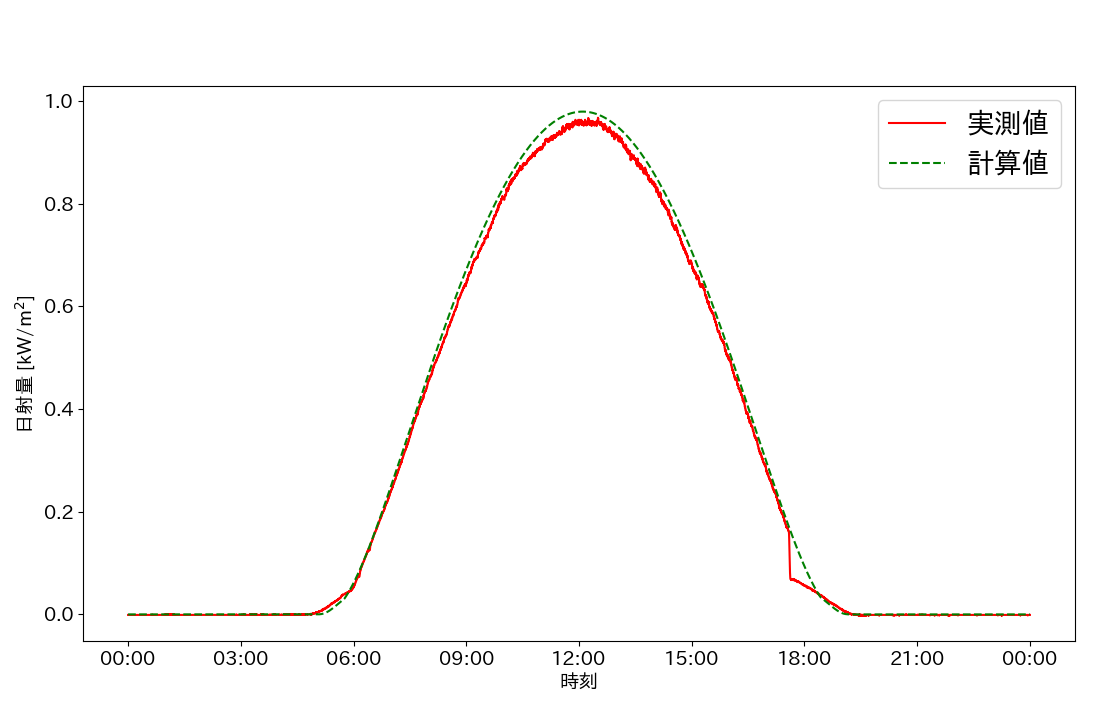
\includegraphics[width=160mm]{sotu/figure/2/pvlib-20220602-corr.png}
  \caption{2022年6月2日の実測値と地表日射量(pvlib値)}
  \label{2-p1}
\end{figure}

\subsection{地表日射量との相互相関による時刻補正法}
相互相関の計算に使用した期間は図\ref{20220529-p1}と同じ2022年6月2日0時0分から2022年6月2日23時59分とした.

この期間の地表日射量を求め, 相互相関を計算した結果, 実測値を121秒遅らせた際に, 相関が最大となることが分かった.  また, 2022年5月3日と2022年5月18日ではそれぞれ26秒, 59秒遅らせた際に相関が最大となり, 3日間の平均値は68秒であった.

式(2.1)~式(2.7)より求めた大気外日射量を用いて相互相関を計算した時と比較して, 78秒から68秒へと10秒改善した.

\section{前処理の追加による時刻補正法とその精度}

図\ref{2-p1}では, 日の入時刻の辺りにおいて, 実測値と地表日射量の概形が大きく異なっている.

太陽光パネルの周囲にある建造物の影による実測値のひずみを事前に取り除いた上で相互相関を計算することで, 相互相関の計算結果が改善するかを検証するために, 実測値に対して前処理を追加した.

前処理を含めた相互相関の計算方法は以下の手順で行う.

\begin{enumerate}
  \item 実測値が歪んでいる時間の日射量を0 \si{\kilo\watt}/\si{\metre\squared}と見なすためのしきい値の指定: 本論文では, 0.2 \si{\kilo\watt}/\si{\metre\squared}をしきい値として設定した.
  \item しきい値に該当する計測時刻の特定: 続いて, 実測値の日射量データから0.2 \si{\kilo\watt}/\si{\metre\squared}を減算して絶対値を取った際に最も0に近い値を取る計測時刻を午前と午後でそれぞれ一点ずつ特定した.
  \item 特定した計測時刻を使った実測値のフィルタリング: 前のステップで得た計測時刻を使用して, 2点の計測時刻の外側にある実測値の日射量を0 \si{\kilo\watt}/\si{\metre\squared}とした.
  \item 地表日射量との相互相関の計算: 実測値の歪み部分を0 \si{\kilo\watt}/\si{\metre\squared}とした後, 地表日射量との相互相関を計算した.
\end{enumerate}

図\ref{2-p2}に, この前処理を行ったリサイクル館の実測値と地表日射量を比較する.

なお, 図\ref{2-p2}は\texttt{python3 selective_corr.py -dt 2022/06/02 -slide_seconds 0 -surface_tilt 22 -surface_azimuth 179 -threshold_q 0.2 -show_preprocessing_data \\ -show_threshold_q}コマンドを実行してプロットしている.

\begin{figure}[H]
  \begin{center}
    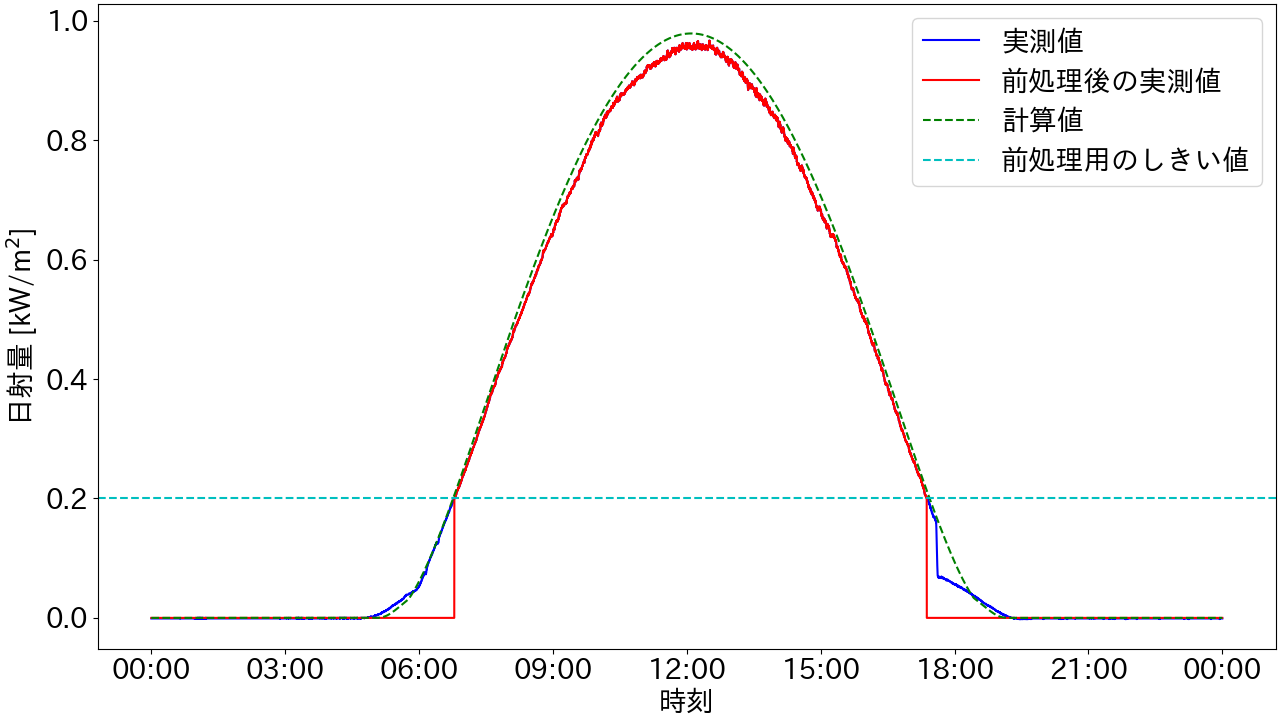
\includegraphics[width=140mm]{sotu/figure/2/drop-under-0.2-q.png}
    \caption{前処理を行った2022年6月2日の実測値と地表日射量(計算値)}
    \label{2-p2}
  \end{center}
\end{figure}

前処理を行った実測値と, 地表日射量から相互相関を計算した結果, 実測値を70秒遅らせた際に, 相関が最大となった. また, 2022年5月3日は21秒進めた際に相関が最大となり, 2022年5月18日は12秒遅らせた際に相関が最大となった. 3日間の平均値は34秒であった.

前処理を追加したことで相互相関の結果が, 68秒から34秒へと34秒改善した.

\section{結言}
本章では太陽光発電データの計測時刻の補正手法を提案した. その結果, 前処理を追加したことで相互相関の結果が68秒から34秒に改善した.

次章では本章で述べた2年分のデータを蓄積している単一Elasticsearchノードをクラスタ化する前に行うデータ移行手法について述べる.